\documentclass[aspectratio=169]{beamer}

\usetheme{Boadilla}
\usefonttheme{professionalfonts}
\setbeamertemplate{navigation symbols}{}
\setbeamertemplate{itemize items}[circle]
\setbeamertemplate{enumerate items}[default]
\setbeamertemplate{headline}{}

\usepackage[utf8]{inputenc}
\usepackage[T1]{fontenc}
\usepackage{lmodern}
\usepackage{amsmath}
\usepackage{booktabs}
\usepackage{tabularx}
\usepackage{array}
\usepackage{hyperref}
\usepackage[strings]{underscore}
\usepackage{listings}
\usepackage{tikz}
\usetikzlibrary{arrows.meta,positioning,fit,calc,shapes.geometric}
\usepackage{xcolor}

\definecolor{courseblue}{HTML}{12355B}
\definecolor{coursegold}{HTML}{C98A2E}
\definecolor{courseice}{HTML}{EEF3F8}
\definecolor{coursegreen}{HTML}{2F6B4F}
\definecolor{coursegray}{HTML}{4B5563}
\definecolor{codebg}{HTML}{F7F9FC}
\definecolor{codecomment}{HTML}{5E6C84}
\definecolor{codestring}{HTML}{0B6E4F}

\setbeamercolor{palette primary}{bg=courseblue,fg=white}
\setbeamercolor{palette secondary}{bg=coursegold,fg=white}
\setbeamercolor{palette tertiary}{bg=courseblue,fg=white}
\setbeamercolor{palette quaternary}{bg=coursegold,fg=white}
\setbeamercolor{structure}{fg=courseblue}
\setbeamercolor{frametitle}{bg=courseice,fg=courseblue}
\setbeamercolor{title}{fg=courseblue}
\setbeamercolor{block title}{bg=courseblue,fg=white}
\setbeamercolor{block body}{bg=courseice,fg=black}
\setbeamercolor{normal text}{fg=black,bg=white}
\setbeamercolor{alerted text}{fg=coursegold}

\setbeamerfont{footline}{size=\scriptsize}

\setbeamertemplate{footline}{
  \leavevmode
  \hbox{
    \begin{beamercolorbox}[wd=.33\paperwidth,ht=2.8ex,dp=1.2ex,leftskip=0.8em]{palette primary}%
      University of Trieste
    \end{beamercolorbox}%
    \begin{beamercolorbox}[wd=.49\paperwidth,ht=2.8ex,dp=1.2ex,center]{palette tertiary}%
      \coursename{} \textbar{} \coursecode
    \end{beamercolorbox}%
    \begin{beamercolorbox}[wd=.18\paperwidth,ht=2.8ex,dp=1.2ex,rightskip=0.8em plus1fil]{palette secondary}%
      \insertframenumber{} / \inserttotalframenumber
    \end{beamercolorbox}%
  }
}

\hypersetup{
  colorlinks=true,
  linkcolor=courseblue,
  urlcolor=coursegreen
}

\lstdefinestyle{coursepython}{
  language=Python,
  basicstyle=\ttfamily\footnotesize,
  keywordstyle=\color{courseblue}\bfseries,
  commentstyle=\color{codecomment}\itshape,
  stringstyle=\color{codestring},
  showstringspaces=false,
  columns=fullflexible,
  keepspaces=true,
  frame=single,
  framerule=0.6pt,
  rulecolor=\color{courseblue},
  backgroundcolor=\color{codebg},
  xleftmargin=0.4em,
  xrightmargin=0.4em,
  aboveskip=0.4em,
  belowskip=0.2em
}

\newcommand{\coursename}{Data-driven Systems Engineering}
\newcommand{\coursecode}{440MI / 305SM}
\newcommand{\coursefooter}{}

\newcommand{\learninggoals}[1]{
  \begin{block}{Learning goals}
  #1
  \end{block}
}

\newcommand{\repoactivity}[1]{
  \begin{block}{Repo activity}
  #1
  \end{block}
}

\newcommand{\readinglist}[1]{
  \begin{block}{Papers and materials}
  {\footnotesize #1}
  \end{block}
}

\newcommand{\coursecontextframe}[5]{
  \begin{frame}{Course Map and Running Cases}
  \centering
  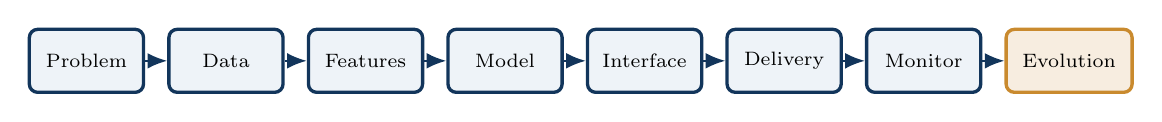
\begin{tikzpicture}[node distance=0.28cm]
  \node[flowbox, minimum width=1.45cm, minimum height=0.8cm] (problem) {\scriptsize Problem};
  \node[flowbox, minimum width=1.45cm, minimum height=0.8cm, right=of problem] (data) {\scriptsize Data};
  \node[flowbox, minimum width=1.45cm, minimum height=0.8cm, right=of data] (features) {\scriptsize Features};
  \node[flowbox, minimum width=1.45cm, minimum height=0.8cm, right=of features] (model) {\scriptsize Model};
  \node[flowbox, minimum width=1.45cm, minimum height=0.8cm, right=of model] (interface) {\scriptsize Interface};
  \node[flowbox, minimum width=1.45cm, minimum height=0.8cm, right=of interface] (delivery) {\scriptsize Delivery};
  \node[flowbox, minimum width=1.45cm, minimum height=0.8cm, right=of delivery] (monitor) {\scriptsize Monitor};
  \node[accentbox, minimum width=1.6cm, minimum height=0.8cm, right=of monitor] (evolution) {\scriptsize Evolution};
  \foreach \a/\b in {problem/data,data/features,features/model,model/interface,interface/delivery,delivery/monitor,monitor/evolution} {
    \draw[arrow] (\a) -- (\b);
  }
  \end{tikzpicture}

  \vspace{0.5em}
  \begin{block}{Today in the course}
  \textbf{Focus:} #1

  \textbf{Bridge:} #2
  \end{block}

  \begin{columns}[T]
  \column{0.48\textwidth}
  \begin{block}{Fraud case}
  {\footnotesize #3}
  \end{block}
  \column{0.48\textwidth}
  \begin{block}{Pasteurization case}
  {\footnotesize #4}
  \end{block}
  \end{columns}

  \vspace{0.3em}
  {\footnotesize \textbf{Course thread:} #5}
  \coursefooter
  \end{frame}
}

\newcommand{\classclosingframe}[4]{
  \begin{frame}{From This Class to the Next}
  \begin{block}{What stays with us}
  #1
  \end{block}

  \begin{columns}[T]
  \column{0.48\textwidth}
  \begin{block}{Project use}
  {\footnotesize #2}
  \end{block}
  \column{0.48\textwidth}
  \begin{block}{Next connection}
  {\footnotesize #3}
  \end{block}
  \end{columns}

  \vspace{0.3em}
  {\footnotesize \textbf{Course thread:} #4}
  \coursefooter
  \end{frame}
}

\tikzset{
  flowbox/.style={
    rounded corners=3pt,
    draw=courseblue,
    fill=courseice,
    very thick,
    minimum width=2.2cm,
    minimum height=0.9cm,
    align=center,
    font=\small
  },
  accentbox/.style={
    rounded corners=3pt,
    draw=coursegold,
    fill=coursegold!15,
    very thick,
    minimum width=2.2cm,
    minimum height=0.9cm,
    align=center,
    font=\small
  },
  arrow/.style={
    -{Latex[length=2.5mm,width=2mm]},
    thick,
    draw=courseblue
  }
}


\title{Class 16: Modeling Fundamentals, Experiment Tracking, and Tuning}
\author{\coursename}
\date{}

\begin{document}

\frame{\titlepage \coursefooter}

\begin{frame}{Agenda}
\begin{itemize}
\item Modeling as abstraction and representation choice.
\item Matching model families to problem types and constraints.
\item Why experimentation is engineering practice, not casual score-hunting.
\item What must be tracked to compare models fairly.
\item Tuning strategies and Neptune-style experiment logging in this repository.
\item From a tuned run to a governed, traceable artifact.
\end{itemize}
\coursefooter
\end{frame}

\begin{frame}{Learning goals}
\learninggoals{
\begin{itemize}
\item Frame modeling as an engineering choice among accuracy, interpretability, speed, and maintainability.
\item Match model families to data, objectives, and operational constraints.
\item Design an experiment before running it, and know what must be logged to compare runs fairly.
\item Explain how hyperparameter search connects to reproducibility and later delivery.
\end{itemize}
}
\coursefooter
\end{frame}

\coursecontextframe
{Choosing model families and turning experimentation into a disciplined, tracked practice.}
{With features settled, this class asks how to compare modeling choices honestly, and how to keep evidence for why one model was selected over another.}
{In the fraud case, we compare model families and hyperparameters for a rare-event classifier and log every run so results stay reproducible.}
{In the pasteurization case, experiment tracking can compare forecasting variants or preprocessing choices without losing context between runs.}
{A good model choice must be explainable, repeatable, and ready for later delivery, not just the best number in a notebook.}

\begin{frame}{What is modeling?}
\begin{itemize}
\item Modeling represents patterns in data so the system can generalize to unseen cases.
\item Every model encodes assumptions about structure, noise, and decision boundaries.
\item Choosing a model means choosing a trade-off among accuracy, interpretability, speed, and maintainability.
\end{itemize}
\coursefooter
\end{frame}

\begin{frame}{Useful modeling questions}
\begin{enumerate}
\item What decision or prediction are we supporting?
\item What kind of target do we have: class, score, or continuous value?
\item What kinds of errors are expensive?
\item How fast must training and inference be?
\item How often do we expect the data distribution to change?
\end{enumerate}
\coursefooter
\end{frame}

\begin{frame}{Model families in context}
\begin{tabularx}{\textwidth}{>{\bfseries}l X}
Linear models & Fast, simple, and often strong baselines. \\
Tree-based models & Good for heterogeneous tabular data and nonlinearity. \\
Probabilistic models & Useful when uncertainty and conditional structure matter. \\
Neural networks & Powerful for large unstructured or highly nonlinear problems. \\
Online models & Update incrementally as new observations arrive. \\
\end{tabularx}
\coursefooter
\end{frame}

\begin{frame}{More realistic examples}
\begin{itemize}
\item Fraud detection: random forest or gradient boosting with threshold tuning.
\item Wine-quality-style regression: gradient boosting tuned by grid search and tracked in Neptune.
\item Pasteurization forecasting: incremental regression, revisited fully in Class 18.
\item Industrial anomaly detection: useful only if alert cost and false-positive rate are understood upfront.
\end{itemize}
\coursefooter
\end{frame}

\begin{frame}[fragile]{Repository example: a baseline training pipeline}
\begin{lstlisting}[style=coursepython]
X_train, X_test, y_train, y_test = train_test_split(
    X, y, test_size=0.2, random_state=42, stratify=y
)

scaler = StandardScaler()
X_train_scaled = scaler.fit_transform(X_train)
X_test_scaled = scaler.transform(X_test)
\end{lstlisting}
\begin{itemize}
\item From `streamlit/modeling.py`, mirrored in `notebooks/Class6_Model_Training_.ipynb`.
\item Stratification matters because fraud is rare; a naive split can distort the class balance a model actually sees during training.
\end{itemize}
\coursefooter
\end{frame}

\begin{frame}{Experimentation is an engineering discipline}
\begin{itemize}
\item The purpose of experimentation is not to collect many scores, but to support a credible model choice.
\item Every run should answer a question: does a new feature help, does a different model family help, or does tuning justify extra complexity?
\item Fix the evaluation protocol and decide what counts as a meaningful improvement before looking at results.
\item When the question is unclear, experiment tracking becomes a storage system for confusion rather than evidence.
\end{itemize}
\coursefooter
\end{frame}

\begin{frame}{What must be tracked, and why}
\begin{tabularx}{\textwidth}{>{\bfseries}l X}
Dataset version / extraction date & So a result can be reproduced against the same data later. \\
Feature pipeline version & So preprocessing changes are not confused with model changes. \\
Hyperparameters and seeds & So the exact configuration that produced a result is known. \\
Metrics, confusion matrices, artifacts & So the trained output, not just a number, can be audited. \\
Code commit or notebook snapshot & So the logic behind a run can be replayed months later. \\
\end{tabularx}
\coursefooter
\end{frame}

\begin{frame}{Fair comparison versus common bias}
\begin{columns}[T]
\column{0.48\textwidth}
\textbf{A fair comparison has}
\begin{itemize}
\item The same dataset split or protocol
\item The same preprocessing, unless that is the experiment
\item Metrics chosen for the real decision
\end{itemize}
\column{0.48\textwidth}
\textbf{Bias creeps in from}
\begin{itemize}
\item Reusing the test set until it becomes part of tuning
\item Mixing notebook state and hidden edits
\item Reporting only the winning run
\end{itemize}
\end{columns}
\coursefooter
\end{frame}

\begin{frame}{Model search strategies}
\begin{tabularx}{\textwidth}{>{\bfseries}l X}
Manual tuning & Small problems and pedagogical intuition. \\
Grid search & Small, well-structured search spaces. \\
Random search & Better coverage when many hyperparameters matter unevenly. \\
Bayesian optimization & Expensive models where each run has high cost. \\
\end{tabularx}
\vspace{0.4em}
\begin{itemize}
\item A tuned model should beat a simple, previously deployed, or default baseline by a meaningful margin, not just a decimal point.
\end{itemize}
\coursefooter
\end{frame}

\begin{frame}[fragile]{Neptune example: defining a search space}
\begin{lstlisting}[style=coursepython]
model = GradientBoostingRegressor(random_state=42)

param_grid = {
    "n_estimators": [100, 200, 300],
    "max_depth": [3, 5, 7],
    "learning_rate": [0.05, 0.1, 0.2],
    "min_samples_split": [2, 5, 10],
}
\end{lstlisting}
\begin{itemize}
\item From `notebooks/Class7_Model_Tuning_Neptune.ipynb`, which uses the Neptune.ai experiment tracker alongside `GridSearchCV`.
\item The grid gives a realistic trade-off among model complexity, fit time, and predictive gain.
\end{itemize}
\coursefooter
\end{frame}

\begin{frame}[fragile]{Neptune example: tuning and logging together}
\begin{lstlisting}[style=coursepython]
grid_search.fit(X_train, y_train)

run["best/parameters"] = grid_search.best_params_
run["best/cv_score"] = grid_search.best_score_
\end{lstlisting}
\begin{itemize}
\item The important idea is not Neptune specifically, but the discipline of storing parameters and metrics together, in the same place, automatically.
\item That same pattern maps naturally onto MLflow, Weights \& Biases, or an internal experiment registry.
\end{itemize}
\coursefooter
\end{frame}

\begin{frame}{From notebook run to governed asset}
\centering
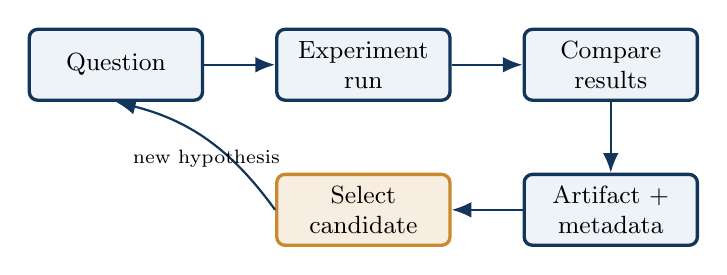
\begin{tikzpicture}[node distance=0.9cm and 0.9cm]
\node[flowbox] (question) {Question};
\node[flowbox, right=of question] (run) {Experiment\\run};
\node[flowbox, right=of run] (compare) {Compare\\results};
\node[flowbox, below=of compare] (artifact) {Artifact +\\metadata};
\node[accentbox, left=of artifact] (select) {Select\\candidate};
\draw[arrow] (question) -- (run);
\draw[arrow] (run) -- (compare);
\draw[arrow] (compare) -- (artifact);
\draw[arrow] (artifact) -- (select);
\draw[arrow, bend right=20] (select.west) to node[below, font=\scriptsize] {new hypothesis} (question.south);
\end{tikzpicture}
\coursefooter
\end{frame}

\begin{frame}[fragile]{Neptune example: evaluate and persist the winner}
\begin{lstlisting}[style=coursepython]
best_model = grid_search.best_estimator_
y_pred = best_model.predict(X_test)

run["test/mse"] = mean_squared_error(y_test, y_pred)
run["test/r2"] = r2_score(y_test, y_pred)

joblib.dump(best_model, "best_gb_model.pkl")
run["artifacts/model"].upload("best_gb_model.pkl")
\end{lstlisting}
\begin{itemize}
\item A useful experiment ends with a traceable artifact, not only a screenshot of the best score.
\item This is also the natural bridge to model registries and deployment, covered fully in Class 20.
\end{itemize}
\coursefooter
\end{frame}

\begin{frame}{Common tuning mistakes}
\begin{itemize}
\item Tuning on the test set.
\item Comparing runs trained on different preprocessing logic.
\item Reporting only the best metric, not its variability or computational cost.
\item Forgetting that a slightly weaker model may be much easier to deploy, explain, or monitor.
\end{itemize}
\coursefooter
\end{frame}

\begin{frame}{Repository connections}
\repoactivity{
\begin{itemize}
\item `notebooks/Class6_Model_Training_.ipynb` gives the baseline split, tune, evaluate, and serialize workflow.
\item `notebooks/Class7_Model_Tuning_Neptune.ipynb` adds Neptune.ai tracking on top of the same grid-search pattern.
\item Together they show the same discipline applied with and without an experiment tracker.
\end{itemize}
}
\coursefooter
\end{frame}

\begin{frame}{Discussion prompt}
\begin{block}{Question}
Two runs report similar cross-validation scores but were trained on differently scaled inputs. Can we trust the comparison?
\end{block}
\begin{itemize}
\item This connects tracked metadata directly back to the ``what must be tracked'' table earlier in this class.
\end{itemize}
\coursefooter
\end{frame}

\begin{frame}{Papers and materials}
\readinglist{
\href{https://docs.neptune.ai/}{Neptune documentation};\
\href{https://mlflow.org/docs/latest/index.html}{MLflow documentation};\
\href{https://scikit-learn.org/stable/modules/grid_search.html}{scikit-learn model selection guide};\
\href{https://jmlr.org/papers/volume13/bergstra12a/bergstra12a.pdf}{Bergstra and Bengio (2012), Random Search};\
\href{https://proceedings.mlr.press/v28/bergstra13.html}{Bergstra et al. (2013), Hyperopt}.
}
\coursefooter
\end{frame}

\classclosingframe
{\begin{itemize}
\item Model selection is tied to the prediction task, the error costs, and the constraints of the system it will live in.
\item A useful experiment records data, configuration, metrics, and artifacts together, automatically.
\item Hyperparameter search is valuable only when it is reproducible, comparable, and beats a real baseline.
\end{itemize}}
{Project teams should now be able to defend a baseline, compare tracked alternatives, and explain why a chosen model fits the fraud or pasteurization setting.}
{Class 17 turns these tracked results into evaluation and decision-making: metrics that reflect the real task, and interfaces that turn a score into an action.}
{Reproducible experimentation is what makes the next step, judging a model's real-world decision quality, meaningful rather than anecdotal.}

\end{document}
